% !TEX encoding = UTF-8
% !TEX program = pdflatex
% !TEX root = relazione.tex
% !TeX spellcheck = it_IT

% ESEMPI
\section{Esempi}\label{sec:esempi}
Parlando di riconoscimenti visivo, è naturale inserire anche alcuni esempi su immagini di prova per mettere a confronto
le diverse piattaforme nei casi specifici.
Sono state identificate quattro funzionalità presenti in tutti i servizi (come si può vedere dalla tabella~\ref{tab:riass-funzionalita} in appendice):
riconoscimento di oggetti specifici, il riconscimento di scene e il riconscimento di volti.

Per consentire la maggior imparzialità, le immagini sono state selezionate casualmente da alcuni motori di ricerca.
%
\subsection{Riconoscimento di un oggetto specifico}\label{subsec:riconscimento-oggetto-specifico}
L'immagine presa come riferimento è la figura~\ref{fig:scontrino} che raffigura uno scontrino fiscale.
\begin{figure}[!h]
\begin{center}
	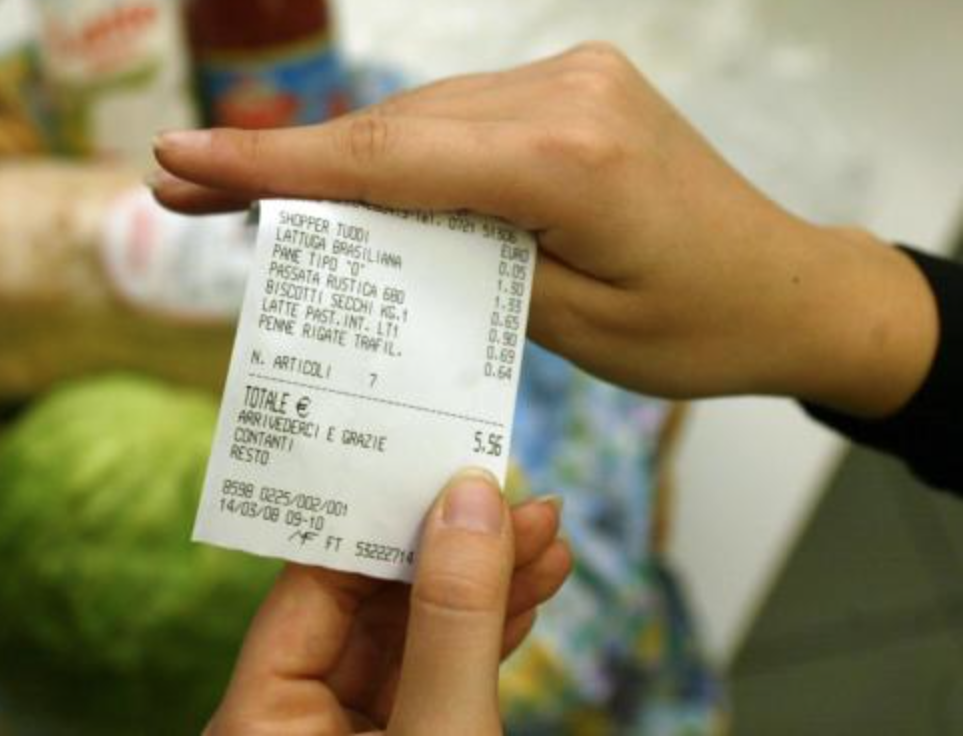
\includegraphics[scale=.5]{scontrino.png}
{\scriptsize \caption{Immagine usata come riferimento.}
\label{fig:scontrino}}
\end{center}
\end{figure}
%
\paragraph{Microsoft} Utilizzando le Computer Vision API con i metodi di tagging, classificazione e generazione di descrizioni,
il risultato ottenuto è:

\label{lst:risultati-microsoft}
\begin{lstlisting}[style=myJSON]
{
   'categories':[
      {
         'name':'text_men',
         'score':0.85546875
      }
   ],
   'description':{
      'captions':[
         {
            'confidence':0.6941834877564524,
            'text':'a close p of a receipt'
         }
      ],
      'tags':[
         'text',
         'receipt'
      ]
   },
   'metadata':{
      'format':'Jpeg',
      'height':450,
      'width':270
   },
   'reqestId':'7249a5f3-3129-4821-aae1-d767a4a3140a',
   'tags':[
      {
         'confidence':0.9944400787353516,
         'name':'text'
      },
      {
         'confidence':0.9528059959411621,
         'name':'receipt'
      }
   ]
}
\end{lstlisting}
